\documentclass{acm_proc_article-sp}

\usepackage{float}
\usepackage{graphicx}
\usepackage[utf8]{inputenc}
\usepackage{listings}

\lstset
{
    basicstyle=\ttfamily\small,
    breakatwhitespace=false,
    breaklines=true,
    frame=single,
    inputencoding=utf8,
    language=bash,
    numbers=left
}

\newcommand{\code}[1]{{\tt #1}}
\newcommand{\prog}[1]{{\tt #1}}

\newcommand{\secref}[1]{(see section \ref{#1})}
\newcommand{\figref}[1]{(see figure~\ref{#1})}

\begin{document}

\title{Datanet Assignment 2}
\subtitle{Webserver}

\numberofauthors{1}
\author{
    \alignauthor
    Casper B. Hansen\\
    \affaddr{University of Copenhagen}\\
    \affaddr{2100 Universitetsparken 5}\\
    \affaddr{Copenhagen, Denmark}\\
    \email{fvx507@alumni.ku.dk}
}

\date{\today}

\maketitle
\begin{abstract}
    Leading into a discussion on the design of the system, I shed light on how
    my initial thoughts and approach. The design stage is followed in
    chronological with considerations put forth along the way, so as to allow
    the reader to understand the rationale behind its conclusions. Lastly, we
    take a look at the extensibility of the system, and how this translates
    into scheduled changes to the system implementation.
\end{abstract}

% A category with the (minimum) three required fields
% \category{H.4}{Information Systems Applications}{Miscellaneous}
% A category including the fourth, optional field follows...
% \category{D.2.8}{Software Engineering}{Metrics}[complexity measures, performance measures]

\terms{Experimentation, Measurement}
\keywords{Web, Server, Protocol}

\section{Overview}
\label{sec:overview}
For the implementation assignments I chose an object-oriented language that
is compiled into machine code and thus executed directly by the CPU, making it
both fast and extensible for further development on later assignments.

\begin{tabular}{ll}
    {\bf Languages}     & C / C++ \\
    {\bf Libraries}     & BSD Sockets (\code{<sys/socket.h>}) \\
\end{tabular}

By choosing a common language, like C++, and using a standard UNIX library,
the server should compile and run on any UNIX system. Considerations were made
to add support for Windows systems, but discarded due to time constraints and
because I didn't have a Windows environment to test against available. Such
cross-platform support could be added using the Winsock library.

\section{Design}
\label{sec:design}
After gaining some basic knowledge of the API I went on to build a crude
program based on what I had learned. Once a working socket program was in
place, I turned what was initially pure C-code into classes and went on to
design the program logic that would drive the web server.

\subsection{Initial Considerations}
I began by analyzing various sources of BSD socket programming examples
online. Since I had no prior experience with BSD sockets this served to gain
an overview of potential class hierarchies. Fortunately, it seems that it
didn't need to be as complicated as I had initially thought it to be.

Inspired by a particular\footnote{BSD http://tldp.org/LDP/LG/issue74/tougher.html}
example, I decided to follow most of its principles almost to the letter, as
I wanted to keep the socket-side programming as simple as possible, and this
code provided just that. Slight optimizations were made, but most of the socket
classes is creditted to this resource. This makes up the socket layer of the
design \figref{fig:design}.

\begin{figure}[H]
    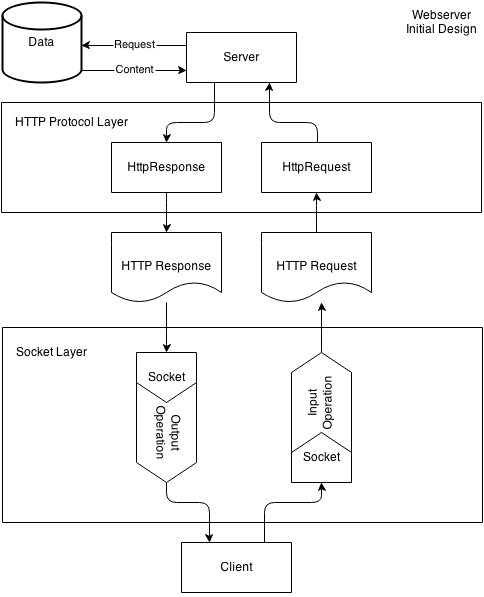
\includegraphics[scale=0.5]{figures/design.png}
    \caption{Initial webserver design}
    \label{fig:design}
\end{figure}

\balancecolumns

\section{Preliminary Design}
\label{sec:design|sub:preliminary-design}
Having a simple socket back-end in place, I began sketching out a class that
would handle the delegation of work and data communication across subsequent
class components. The \code{Server} class is the driving component of the
system \figref{fig:design}; it handles initialization, main run-time logic and
exception handling.

At this point, the system was able to send and receive socket messages. The
system is thus far only meant to support the HTTP protocol, and so the
remainder comes down to the two-part task of implementing HTTP messages; 1)
parse and validate received requests, and 2) generate and send an appropriate
response back.

Since HTTP requests and responses do share some common elements (e.g. the HTTP
version), I reason that a superclass (\code{HttpMessage}) might be useful.
Following this, I then subclassed the \code{HttpMessage} into the two classes
\code{HttpRequest} and \code{HttpResponse}, which encapsulate the concepts of
HTTP requests and responses.

The \code{HttpRequest} parses the raw socket data received. Should it be
invalid class throws an \code{HttpException} which that are used for error
responses --- that is, 4xx- and 5xx-HTTP responses (i.e. if the server doesn't
support a given request method). If it is valid, the server then tries to
process the request, formulating an \code{HttpResponse} which is then sent
back to the socket that received the request \figref{fig:design}.

The \code{ServerSocket} was then extended to be able to transmit HTTP messages
via the stream operators --- using \code{{>}{>}} to receive socket data and
\code{{<}{<}} to send socket data.

\subsection{Limitations}
\label{sec:design|sub:limitations}
The system is limited to support only a few of the requests documented in
the HTTP RFC 2616\footnote{HTTP (RFC 2616) ---
{\tt http://www.w3.org/Protocols/rfc2616/rfc2616.html}} specification. A table
of the level of support on each is given below.

\begin{tabular}{ll}
    {\bf GET}       & Partially Supported, minimal use of fields \\
    {\bf HEAD}      & Fully Supported, needs optimization \\
    {\bf DELETE}    & Planned Support, due for 3rd revision \\
    {\bf POST}      & Planned Support, due for 2nd revision \\
    {\bf PUT}       & Planned Support, due for 3rd revision \\
    {\bf OPTIONS}   & Planned Support, no due date set \\
    {\bf CONNECT}   & Not Supported \\
    {\bf TRACE}     & Not Supported \\
\end{tabular}

The \code{GET} request is the most essential, as it provides the server with
information on what the client wishes to access on the server. No server can
function without it, and therefore support for it was implemented.

Since the system is to be extended into a peer-to-peer (or P2P) system, the
\code{HEAD} request was inevitable, as in a P2P system a client may not wish
to download a file, but rather simply want information about it. This is what
the \code{HEAD} request is meant for, and so in preparation of the coming
system extension support for this was added.

\balancecolumns
\subsection{Extensibility}
\label{sec:design|sub:extensibility}
Many considerations went into the initial design of the system, but many were
discarded due to the time constraint. Thus, many design considerations were
jotted down and therefore not a part of this version, but rather subject to
change in the following assignments.

The following discusses each part of the implementation that ought be changed.

\subsubsection{HTTP Messages}
\label{sec:design|sub:extensibility|sub:http-messages}
The abstraction of a generic HTTP message is considered good, but as responses
to different requests vary much in their structure and required data, it may
prove useful to subclass the \code{HttpResponse} into each supported response
(i.e. \code{HttpGetResponse}).

\subsubsection{Generated HTML}
\label{sec:design|sub:extensibility|sub:generated-html}
Some HTTP responses require the generation of HTML content. Such functionality
should be encapsulated in a class. This will probably follow from the HTTP
response subclassing, as discussed \secref{sec:design|sub:extensibility|sub:http-messages}.
Having such a class would make it easier to extend the system in any aspect
that may require server generated content.

\section{Tests}
\label{sec:tests}
Most tests were carried out by accessing the server via the \prog{telnet}.
Unfortunately, I did not have time to show test cases of the exception
handling mechanism, although it does work, and can be verified by compiling
and running the server on the readers own system.

\subsection{GET}
To test the \code{GET} method, we must first ensure that the server can serve
files. In the test below I queried the server for the \code{/sample.txt} file.
It is expected to return an HTTP response with the 200 code, meaning
everything went well, followed by the server name, date, correct MIME-type,
the length of the content and that the server closes the connection.
\begin{figure}[H]
    \lstinputlisting{logs/get-file.log}
    \caption{Response for \code{GET /sample.txt HTTP/1.0}}
    \label{fig:get-file}
\end{figure}

When the server is queried for a directory we want it to serve the
\code{index.html} file, if it exists. The test below shows the server handling
this request.

\balancecolumns

\begin{figure}[H]
    \lstinputlisting{logs/get-index.log}
    \caption{Response for \code{GET / HTTP/1.0}}
    \label{fig:get-index}
\end{figure}

Following up on the previous test, if no such file exists we wish to generate
and serve a list of files in the queried directory. For purposes of testing
this, I renamed the \code{index.html} to \code{\_index.html} temporarily.
\begin{figure}[H]
    \lstinputlisting{logs/get-list.log}
    \caption{Response for \code{GET / HTTP/1.0}, where no \code{index.html} can be found}
    \label{fig:get-list}
\end{figure}

\subsection{HEAD}
In testing the \code{HEAD} request there aren't many cases, we simply expect
the header of a \code{GET} response to be returned. Which is indeed the case,
as shown below.
\begin{figure}[H]
    \lstinputlisting{logs/head-file.log}
    \caption{Response for \code{HEAD /sample.txt HTTP/1.0}}
    \label{fig:head-file}
\end{figure}

\bibliographystyle{abbrv}
\bibliography{sigproc}
\begin{thebibliography}{9}
    
    \bibitem{KR}
        James F. Kurose, Keith W. Ross,\\
        \emph{Computer Networking, A Top-Down Approach},\\
        Pearson Education, Sixth Edition, 2013
    
\end{thebibliography}

\end{document}

